\thispagestyle{toanhocvadoisongnone}
\pagestyle{toanhocvadoisong}
\everymath{\color{toanhocdoisong}}
\graphicspath{{../toanhocdoisong/pic/}}
\begingroup
\blfootnote{$^1$\color{toanhocdoisong}Nguồn: Accromath, vol. $17$, $2022$.}
%\blfootnote{$^2$\color{toanhocdoisong}Đại học McGill, Canada.}
%\blfootnote{$^3$\color{toanhocdoisong}École Polytechnique Fédérale de Lausanne, Thụy Sỹ.}
\blfootnote{$^2$\color{toanhocdoisong}Viện Toán học.}
\blfootnote{$^3$\color{toanhocdoisong}Giải đấu để chọn ra người thách đấu với nhà vô địch -- Pi.}
\AddToShipoutPicture*{\put(0,616){
\includegraphics[width=19.3cm]{../bannertoanhocdoisong}}}
\AddToShipoutPicture*{\put(102,507){
\includegraphics[scale=1]{../tieude.pdf}}}
\centering
\endgroup

\vspace*{200pt}

\begin{multicols}{2}
	\textit{Khi các đấu thủ hoặc các đội thi đấu với nhau, cơ hội chiến thắng của mỗi bên phụ thuộc vào thực lực của họ. Hệ thống tính điểm Elo là một phương pháp tính toán trình độ tương đối của những người chơi trong một trò chơi có tổng bằng không, cho phép đánh giá khả năng về kết cục của một trận đấu.}
	\vskip 0.05cm
	Từ ngày $24$ tháng $11$ đến ngày $16$ tháng $12$ năm $2021$, tại Dubai đã diễn ra giải vô địch thế giới môn cờ vua. Kỳ thủ Nauy Magnus Carlsen, nhà vô địch từ năm $2013$, đấu với kỳ thủ Nga Ian Nepomniachtchi, người giành chiến thắng ở Giải đấu các ứng viên$^{\small{3}}$. Người chiến thắng giành được $1{,}2$ triệu euro tiền thưởng.
	\vskip 0.05cm
	Trận đấu gồm $14$ ván. Mỗi ván thắng được $1$ điểm, thua $0$ điểm và nếu hòa thì mỗi đấu thủ được $\frac{1}{2}$ điểm. Chung cuộc, Carlsen giành chiến thắng $7\frac{1}{2} - 3\frac{1}{2}$, với $4$ thắng, $0$ thua và $7$ hòa sau $11$ ván ($3$ ván cuối cùng không cần thiết vì không làm thay đổi kết quả cuối cùng). Và như vậy Carlsen giành danh hiệu vô địch thế giới lần thứ $5$ liên tiếp.
	\vskip 0.05cm
	Kết quả này phù hợp với hệ thống tính điểm Elo mà Liên đoàn Cờ vua Thế giới (FIDE) sử dụng từ năm $1970$ để đánh giá trình độ tương đối của các kỳ thủ. Quả thực, khi đó Carlsen được xếp hạng số một thế giới với số điểm Elo $2856$, trong khi đối thủ của anh, kỳ thủ số một của Nga, xếp thứ năm với số điểm Elo $2782$.
	\vskip 0.05cm
	Khi hai đấu thủ $A$ và $B$ với Elo $\theta_A$ và $\theta_B$ đấu với nhau, phương pháp Elo dự đoán $A$ sẽ giành được số điểm trung bình là
	\setlength{\abovedisplayskip}{4pt}
	\setlength{\belowdisplayskip}{5pt}
	\begin{align*}
		s_{AB} = \frac{1}{1+ 10^{-(\theta_A - \theta_B) /400}} \tag{$1$}
	\end{align*}
	biết rằng $A$ được $1$ điểm nếu thắng, $0$ nếu thua và $\frac{1}{2}$ nếu hòa. Điểm số trung bình B giành được là $s_{BA} = 1 – s_{AB}$.
	\vskip 0.05cm
	Trước trận tranh ngôi vô địch, ta có $\theta_A = 2856$ với Carlsen và $\theta_B = 2782$ với Nepomniachtchi, do đó $s_{AB} \approx 0{,}60$, tiên đoán chiến thắng của kỳ thủ Nauy vì trung bình anh sẽ giành được $8\frac{1}{2}$ điểm sau $14$ ván, so với số điểm $5\frac{1}{2}$ của kỳ thủ Nga.
	\vskip 0.05cm
	\textbf{\color{toanhocdoisong}Cơ sở toán học của phương pháp tính điểm Elo}
	\vskip 0.05cm
	Để xác định số điểm trung bình $s_{AB}$ của kỳ thủ $A$ khi đấu với kỳ thủ $B$, phương pháp ngây thơ là lấy số điểm trung bình của $A$ trong các trận đã đấu giữa hai người. Nhưng trong một trò chơi như cờ vua, phần lớn trong số hàng trăm nghìn người chơi chưa từng gặp nhau, và ngay cả khi họ đã từng gặp nhau, số trận họ đã đấu với nhau là quá ít để có một đánh giá chất lượng. Hệ thống tính điểm Elo giải quyết khó khăn này dựa vào một mô hình toán học cho phép xếp hạng các đấu thủ và qua đó ước tính kết quả có thể xảy ra khi họ đối đầu nhau.
	\vskip 0.02cm
	Biểu thức ($1$) lấy cảm hứng từ một mô hình được thiết lập từ những năm $1920$ bởi nhà toán học người Đức Ernst Zermelo và sau đó được cải tiến bởi nhà thống kê người Canada Ralph Bradley và người đồng nghiệp Milton Terry. Trong các công trình này, cũng như trong phần còn lại của bài viết, ta giả sử mọi ván đấu đều phân định thắng thua. Như vậy đây là một mô hình đơn giản hóa, nhất là đối với môn cờ vua, khi hòa là kết quả thường xảy ra nhất giữa các kỳ thủ đỉnh cao.
	\vskip 0.02cm
	Khi một ván đấu kết thúc với kết quả thắng $(1)$ hoặc thua $(0)$, điểm số trung bình chính là xác suất $p_{AB}$ để $A$ thắng $B$. Mô hình Bradley--Terry--Elo giả sử rằng xác suất này có dạng
	
	\vspace{-15pt}
	\begin{align*}
		p_{AB} = G(\theta_A - \theta_B)\tag{$2$}
	\end{align*}
	ở đó $G: \mathbb R \rightarrow (0, 1)$ là một hàm liên tục, tăng ngặt sao cho $G(x) + G(-x) = 1$ với mọi số thực $x$ và $G(x) \rightarrow 1$ khi $x \rightarrow \infty$. Một thí dụ về hàm như thế được cho trong Hình $1$. Ta có $p_{AB} + p_{BA} = G(\theta_A - \theta_B) + G(\theta_B - \theta_A) = 1$, không có kết quả hòa. Vì $G(0) = 1/2$, hai đấu thủ có trình độ ngang nhau có xác suất thắng như nhau; hiệu $\theta_A - \theta_B$ càng tăng thì xác suất để $A$ thắng càng lớn, và tiến tới giới hạn bằng $1$, nghĩa là chiến thắng chắc chắn của $A$.
	Lựa chọn phổ biến nhất của $G$ là luật logistic với tham số $\beta > 0$, được định nghĩa bởi
	
	\vspace{-15pt}
	\begin{align*}
		L(x) = \frac{ 1 }{ (1 + e^{-\beta x}) }\tag{$3$}
	\end{align*}
	với mọi $x \in \mathbb R$.
	\begin{figure}[H]
%		\vspace*{5pt}
		\centering
		\captionsetup{labelformat= empty, justification=centering}
		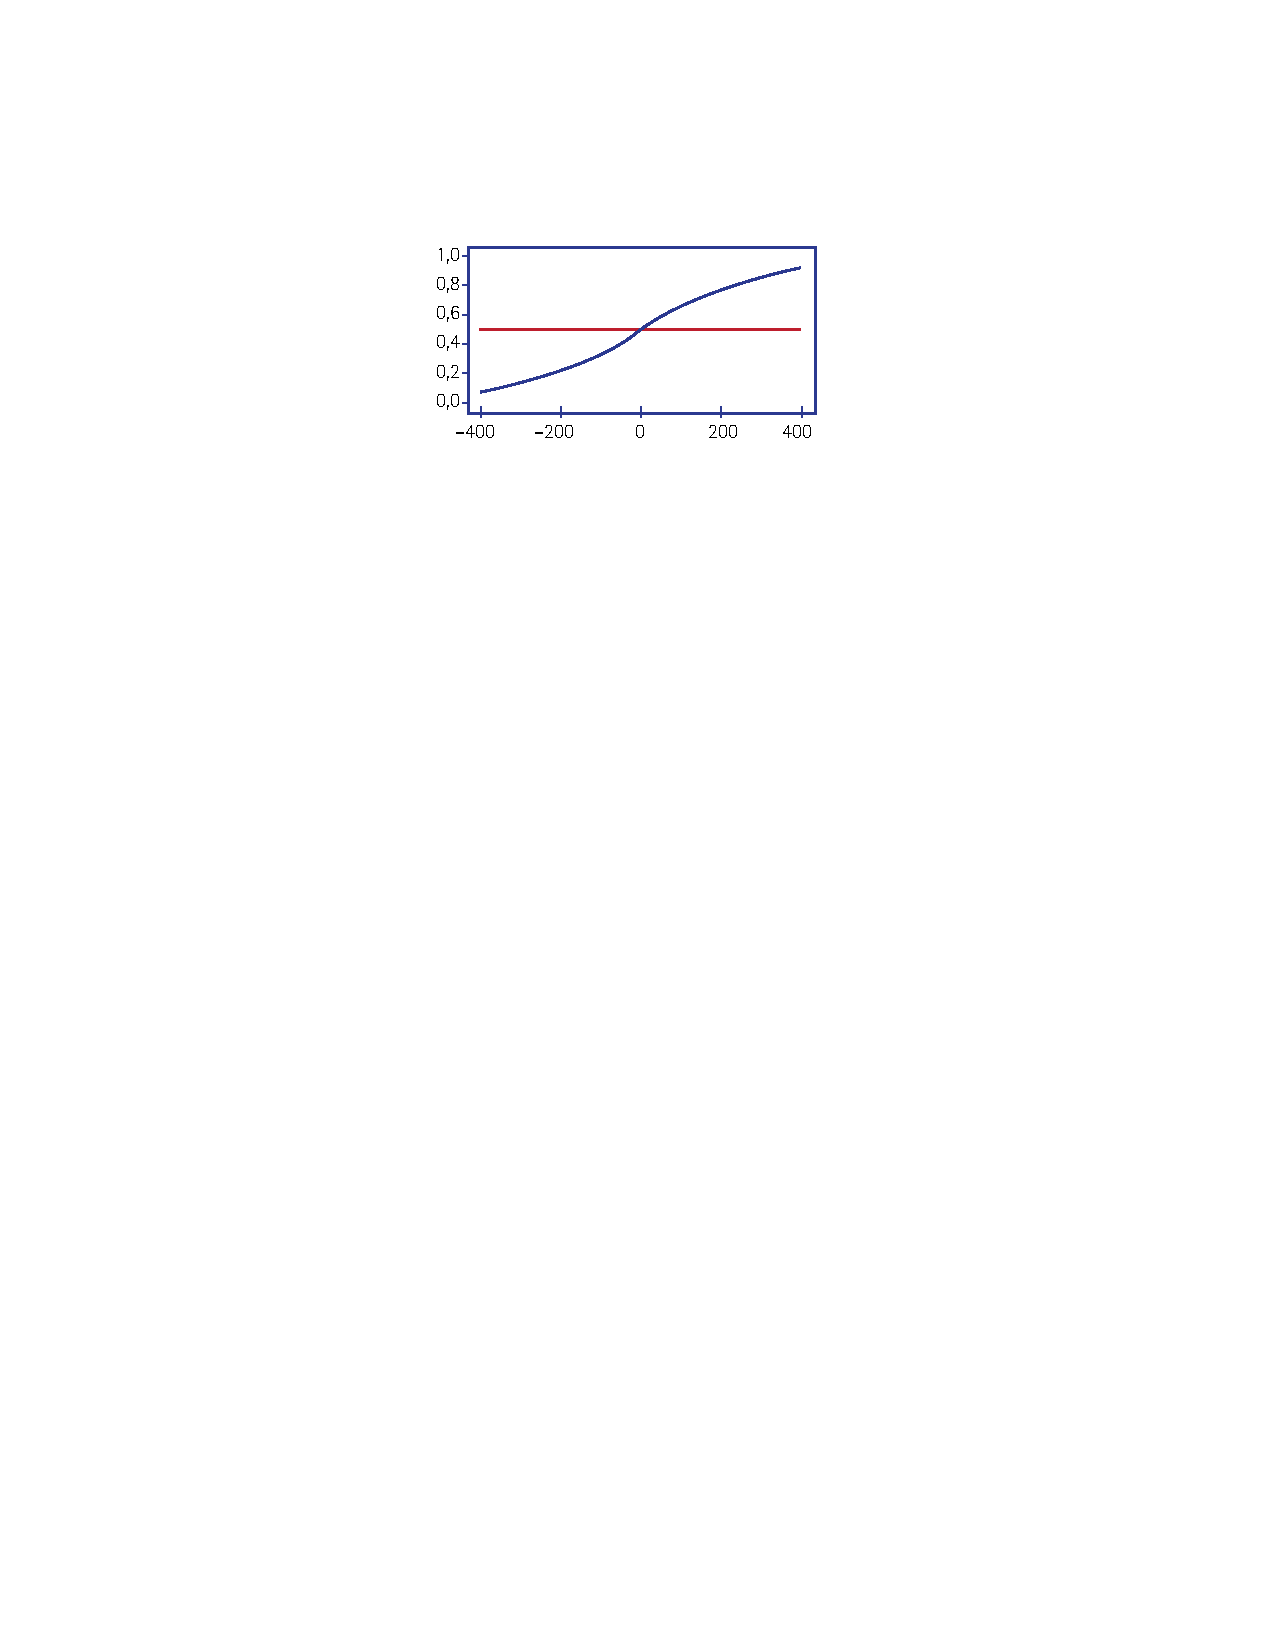
\includegraphics[width= 0.8\linewidth]{pic1}
		\caption{\small\textit{\color{toanhocdoisong}Hình $1$. Đồ thị hàm logistic $L(x)$ với $\beta = \ln(10) / 400$.}}
		\vspace*{-10pt}
	\end{figure}
	Chọn $G = L$ với tham số $\beta = \ln(10) / 400$, ta thu được công thức ($1$) mà FIDE sử dụng. Ban đầu, nhà vật lý người Mỹ gốc Hungary Arpad Elo, người đưa phương pháp mô hình hóa này vào thế giới cờ vua, sử dụng một hàm phân phối chuẩn, khi đó $s_{AB}$ không có công thức tường minh như trên.
	\vskip 0.05cm
	\textbf{\color{toanhocdoisong}Tính chất của mô hình xác suất}
	\vskip 0.05cm
	Mô hình Bradley--Terry--Elo có ưu điểm là nó cho phép xếp hạng tất cả người chơi của một trò chơi theo trình độ tương đối, ngay cả khi họ chưa từng đối đầu trực tiếp. Do đó, ta có thể dùng nó để dự đoán, đặc biệt là dựa vào các mô phỏng.
	Tuy nhiên, giả định rằng xác suất để $A$ thắng $B$ có dạng ($2$) không hề là một điều vô tình. Như đã đề cập, nó ngầm cho rằng không có ván hòa. Nếu có kết quả hòa, mô hình sẽ cần phải được điều chỉnh.
	\vskip 0.05cm
	Biểu thức ($2$) cũng ngầm giả định rằng kết quả một trận đấu giữa $A$ và $B$ chỉ phụ thuộc vào trình độ tương đối $\theta_A - \theta_B$. Đặc biệt, những yếu tố như đi trước (cầm quân trắng trong cờ vua), được nghỉ ngơi nhiều hơn đối thủ, hay thi đấu trước các cổ động viên không ảnh hưởng đến kết quả cuối cùng (một điều không hợp lý đối với thể thao chuyên nghiệp).
	\vskip 0.05cm
	Hơn nữa, cần phải hiểu rằng điểm số Elo của một đấu thủ không hề có giá trị nội tại: ý nghĩa của nó phụ thuộc vào điểm số Elo của các đối thủ, vì ta có thể cộng tất cả với cùng một hằng số tùy ý, hiệu số giữa chúng vẫn giữ nguyên. Tương tự, nếu ta nhân tất cả các Elo với một hằng số $c > 0$ và thay hàm $G(x)$ bởi $G(x / c)$, các xác suất thắng cũng không thay đổi.
	\vskip 0.05cm
	Trong trường hợp công thức ($1$), được biểu diễn trong Hình $1$ với các giá trị $\theta_A - \theta_B$ từ $-400$ đến $+400$, tham số $\beta$ được chọn sao cho chênh lệch $100$ điểm cho xác suất thắng $64\%$ đối với người mạnh hơn. Nếu chênh lệch là $200$ điểm, xác suất là $75\%$, và nó vào khoảng $91\%$ khi chênh lệch là $400$ điểm.
	\vskip 0.05cm
	Trong cờ vua, điểm Elo của hầu hết các kỳ thủ có trong xếp hạng của FIDE nằm trong khoảng từ $1000$ đến $3000$. Phân phối của chúng nói chung không đối xứng và thay đổi tùy theo từng nước. Hơn nữa, có nhiều phiên bản khác nhau của hệ thống xếp hạng, ngoài ra nó còn được điều chỉnh để áp dụng cho nhiều trò chơi và môn thể thao khác, trong đó có cờ vây, \textit{scrabble}, nhiều trò chơi trên mạng, bóng đá, tennis và khúc côn cầu trên băng.
	\vskip 0.05cm
	\textbf{\color{toanhocdoisong}Cập nhật xếp hạng}
	\vskip 0.05cm
	Tất nhiên là trình độ tương đối của các đấu thủ thay đổi theo thời gian. Một số người mạnh lên khi tích lũy thêm kinh nghiệm, một số khác yếu đi do tuổi tác, hoặc, trong trường hợp các môn thể thao đồng đội, do chấn thương, do giải nghệ hoặc do chuyển nhượng không tốt.
	\vskip 0.05cm
	Để thể hiện sự thay đổi này, phương pháp tính điểm Elo đưa ra một quy tắc cập nhật điểm xếp hạng sau mỗi trận đấu. Gọi $\theta_{A, n}$ và $\theta_{B, n}$ là điểm xếp hạng (Elo) của hai đấu thủ A và B ngay trước lần gặp nhau thứ $n$. Elo đề xuất rằng sau trận đấu này, chênh lệch $\theta_{A, n} - \theta_{B, n}$ được phân phối lại cho hai người theo ``độ bất ngờ" của kết quả và một số thực dương $k$, gọi là \textit{hệ số phát triển}.
	\vskip 0.05cm
	Gọi $s$ là kết quả của ván đấu giữa $A$ và $B$, với $s = 1$ nếu $A$ thắng, $s = 0$ nếu $A$ thua và $s = 1/2$ nếu ván đấu hòa. Elo mới của $A$ sẽ là
	\begin{align*}
		\theta_{A, n + 1} = \theta_{A, n} + k (s – s_{AB, n}),
	\end{align*}
	ở đó $s_{AB, n}$ là kết quả dự đoán được tính theo công thức ($1$) với các giá trị $\theta_{A, n}$ và $\theta_{B, n}$. Dễ thấy điểm số Elo của $A$ tăng nếu $s = 1$, và $s_{AB, n}$ càng nhỏ thì điểm số tăng càng nhiều. Như vậy, chiến thắng trước một đối thủ mạnh hơn thì có giá trị hơn. Tương tự, điểm số Elo của $A$ giảm khi thua, tức là khi $s = 0$. Cuối cùng, khi ván đấu hòa, điểm số Elo của $A$ tăng nếu điểm số Elo ban đầu của $B$ lớn hơn, tức là $s_{AB, n} < 1/2$.
	Đối với các kỳ thủ chuyên nghiệp, hệ thống tính điểm Elo cố định giá trị $k = 10$, do đó tại giải vô địch thế giới, mỗi ván thắng mang lại cho Carlsen $10 \times (1 – 0{,}60) \approx 4$ điểm Elo, trong khi mỗi ván hòa khiến anh mất $10 \times (0{,}5 – 0{,}60) \approx 1$ điểm. Sau giải đấu, điểm số Elo mới của anh là
	\begin{align*}
		2856 + 4 \times 4{,}0 - 7 \times 1{,}0 = 2865,
	\end{align*}
	trong khi đó điểm số Elo của Nepomniachtchi giảm từ $2782$ xuống $2773$.
	\vskip 0.05cm
	Các giá trị khác của $k$ được dùng cho các trình độ khác nhau của các kỳ thủ. Chẳng hạn, người ta dùng $k = 40$ cho các kỳ thủ mới chơi chưa quá $30$ ván hoặc các kỳ thủ trẻ dưới $18$ tuổi, giúp họ nhanh chóng đạt đến trình độ thực. Sau đó, $k$ được quy định bằng $20$ chừng nào điểm Elo của họ vẫn ở dưới $2400$.
	\vskip 0.05cm
	\textbf{\color{toanhocdoisong}Tính chất của phương pháp cập nhật}
	\vskip 0.05cm
	Trong trường hợp đặc biệt khi tất cả các ván đấu đều phân thắng bại, ta thấy rằng một cách tổng quát, phương pháp cập nhật mà Elo đề xuất sử dụng một hàm $M: \mathbb R \rightarrow (0, \infty)$ liên tục, giảm ngặt sao cho $M(x) \rightarrow 0$ khi $x \rightarrow \infty$. Hàm này cho phép cập nhật điểm xếp hạng của các đấu thủ $A$ và $B$ như sau.
	\vskip 0.05cm
	Nếu $A$ thắng:
	\begin{align*}
		&\theta_{A, n  +1} = \theta_{A, n} + M(\theta_{A, n} - \theta_{B, n}),\\
		&\theta_{B, n  +1} = \theta_{B, n} - M(\theta_{A, n} - \theta_{B, n}).
	\end{align*}
	Nếu $B$ thắng:
	\begin{align*}
		&\theta_{A, n  +1} = \theta_{A, n} - M(\theta_{B, n} - \theta_{A, n}),\\
		&\theta_{B, n  +1} = \theta_{B, n} + M(\theta_{B, n} - \theta_{A, n}).
	\end{align*}
	Trong công thức của FIDE, $M(x) = k L(-x)$ với mọi số thực $x$.
	\vskip 0.01cm
	Công thức cập nhật này có ý nghĩa tìm kiếm xác suất. Thực vậy, gọi $\theta_A$ và $\theta_B$ là trình độ tương đối thực sự nhưng chưa biết của hai đấu thủ $A$ và $B$. Giả sử $G(\theta_A - \theta_B)$ là xác suất thực sự để $A$ thắng $B$. Kỳ vọng của thay đổi xếp hạng của $A$ tại thời điểm $n$ được cho bởi biểu thức sau:
	\begin{align*}
		&M(\theta_{A, n} - \theta_{B, n}) G(\theta_A - \theta_B)\\
		 &- M(\theta_{B, n} - \theta_{A, n}) G(\theta_B - \theta_A).
	\end{align*}
	Nếu phương pháp cập nhật là tốt, ta mong muốn rằng kỳ vọng này bằng $0$ khi $\theta_{A, n} - \theta_{B, n} = \theta_A - \theta_B$. Do $M$ là hàm giảm, ta cũng hy vọng rằng sau ván đấu, hiệu $(\theta_{A, n + 1} - \theta_{B, n + 1}) - (\theta_A - \theta_B)$ gần $0$ hơn so với hiệu $(\theta_{A, n} - \theta_{B, n}) - (\theta_A - \theta_B)$.
	\vskip 0.01cm
	Lập luận tương tự cũng đúng đối với $B$, và ta có thể kiểm tra rằng những tính chất mong muốn này được đạt nếu các hàm $G$ và $M$ thỏa mãn, với mọi số thực $x$:
	\begin{align*}
		M(x) / M(-x) = G(-x) / G(x). \tag{$4$}
	\end{align*}
	Từ phương trình cân bằng này, với một chút nỗ lực, ta có thể chứng minh rằng với mỗi hàm $M$ cho trước, hàm $G$ duy nhất thỏa mãn được cho bởi
	\begin{align*}
		G(x) = \frac { M(-x) }{ M(x) + M(-x) },
	\end{align*}
	với mọi $x \in \mathbb R$.
	\vskip 0.01cm
	Do đó, quy tắc cập nhật mà Elo đề xuất ngầm cho rằng xác suất ban đầu là xác suất logistic, tức là $G = L$.
	\vskip 0.01cm
	Có một lưu ý tinh tế: nếu ta cố định hàm $G$ trước thì tồn tại vô số hàm $M$ thỏa mãn quan hệ ($4$). Thật vậy, với mọi hằng số $k > 0$, $M(x) = k G(-x)$ là một nghiệm. Nhưng ta cũng có thể chọn $M(x) = k G(-x) S(|x|)$, ở đó $S$ là một hàm thỏa mãn $S(0) = 1$ và $S(x) = S(-x)$ với mọi số thực $x$. Tất nhiên là hàm $S$ được chọn phải đảm bảo tính đơn điệu giảm của $M$.
	\vskip 0.05cm
	\textbf{\color{toanhocdoisong}Kết quả về sự hội tụ}
	\vskip 0.05cm
	Có thể liên hệ phương pháp cập nhật của Elo với thuật toán giảm gradient ngẫu nhiên trong học máy trong một mô hình hồi quy logistic.
	\vskip 0.05cm
	Ta hãy tưởng tượng có $N$ đấu thủ và trình độ của họ được biểu diễn bởi vector $(\theta_1, \dots, \theta_N)$ ẩn nhưng cố định. Ta cũng giả sử rằng ban đầu, ta có một ước lượng $(\theta_{1, 0}, \dots, \theta_{N, 0})$, và các đấu thủ sẽ tham gia một dãy vô hạn các ván đấu, mỗi ván diễn ra 
	\end{multicols}
	\vspace*{-8pt}
	\begin{tBox}
		\begin{wrapfigure}{l}{0.18\linewidth}
			\vspace*{-15pt}
			\centering
			\captionsetup{labelformat= empty, justification=centering}
			\hspace*{3pt}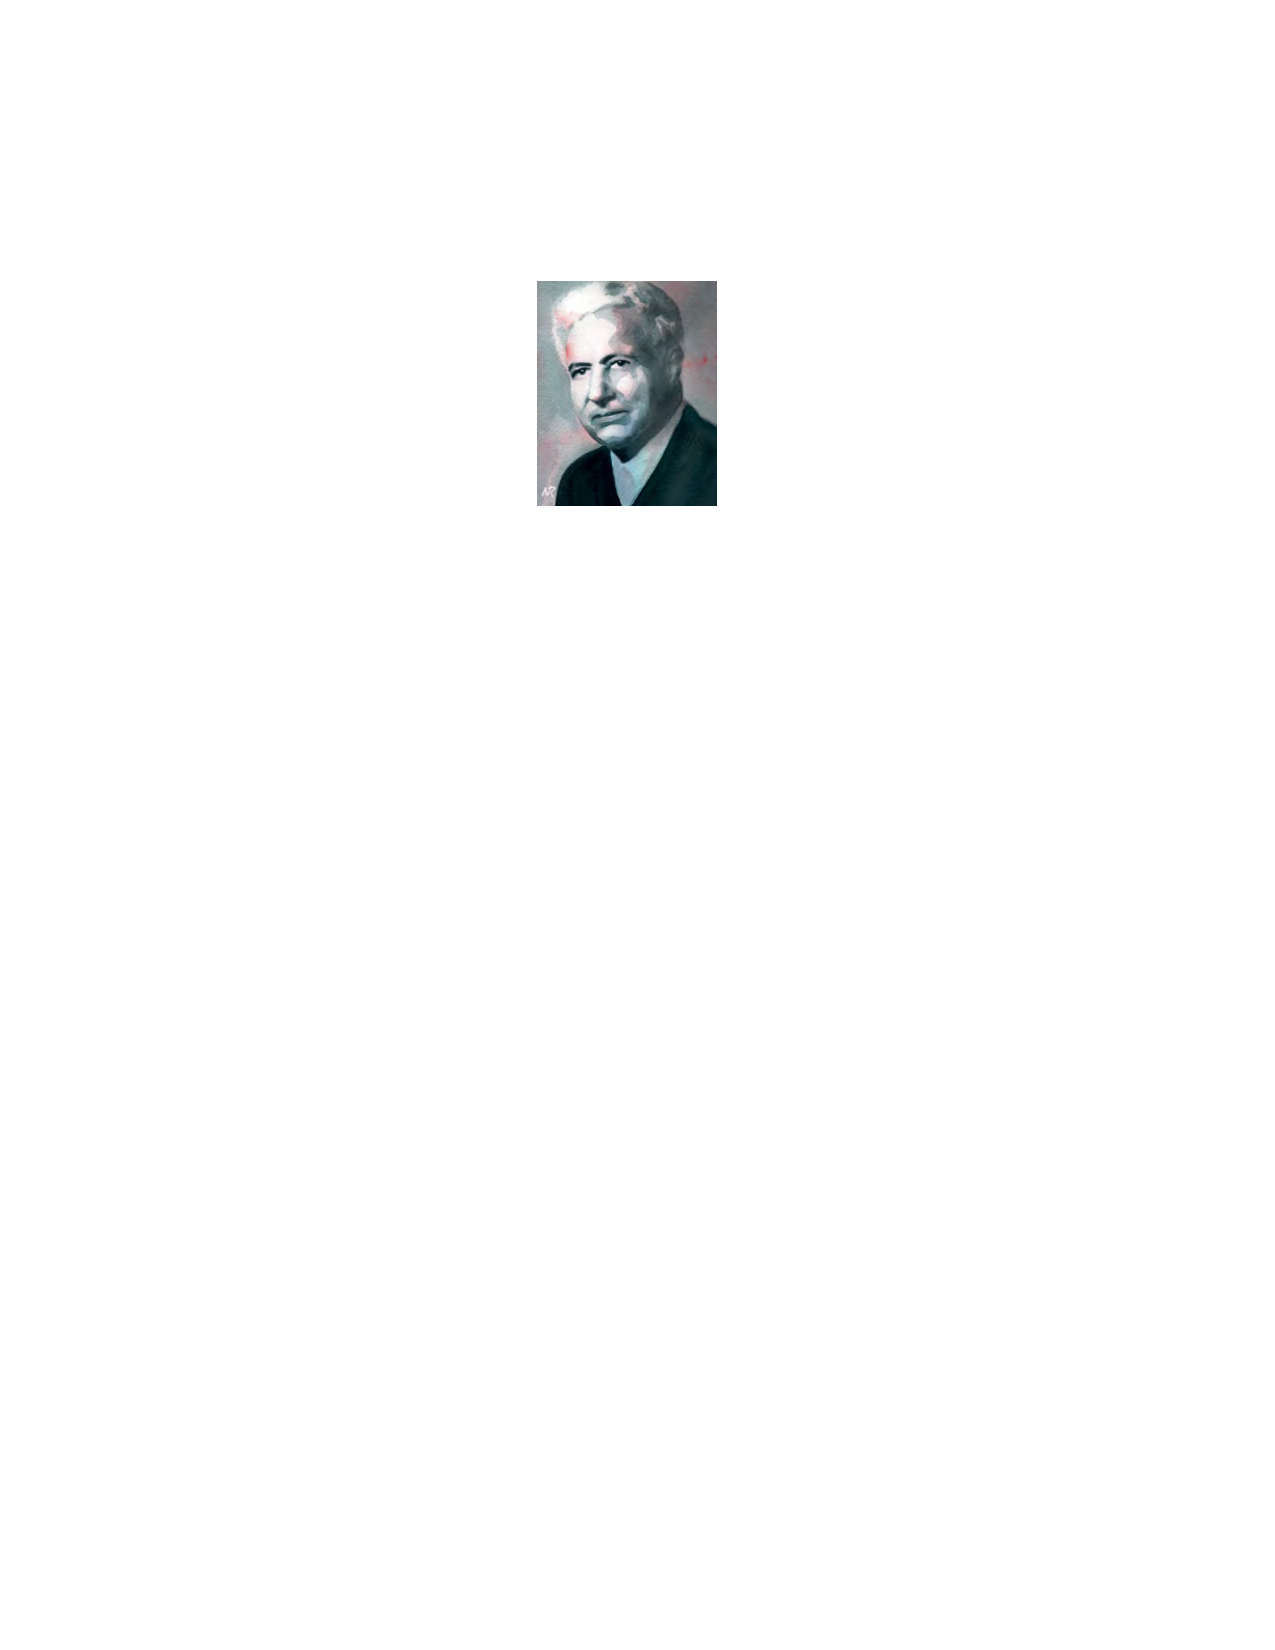
\includegraphics[width= 1.1\linewidth]{pic2}
			\caption{\small\textit{\color{toanhocdoisong}\hspace*{15pt}Arpad Elo.}}
			\vspace*{-20pt}
		\end{wrapfigure}
		Sinh ngày $25$ tháng $8$ năm $1903$ tại Egyházaskeszö, Áo--Hung trong một gia đình khiêm tốn, Arpad Elo (Élö Árpád trong tiếng Hungary) di cư sang Mỹ năm $1913$ cùng cha mẹ. Ông học vật lý tại Đại học Chicago, sau đó giảng dạy tại Đại học Marquette Milwaukee, Wisconsin.
		\vskip 0.05cm
		Ông là một kỳ thủ tài ba, từng tám lần vô địch bang và là chủ tịch Liên đoàn Cờ vua Mỹ từ $1935$ đến $1937$. Ông nổi tiếng thế giới vì đã đưa vào sử dụng hệ thống mang tên mình, được xây dựng trong những năm $1950$ sau khi hệ thống xếp hạng đầu tiên, do Kenneth Harkness phát triển, bị chỉ ra những nhược điểm. Phương pháp mới được FIDE thông qua vào năm $1970$, và Elo trở thành thành viên danh dự của tổ chức này từ năm $1981$.
		\vskip 0.05cm
		Một phân tích chi tiết đầu tiên về hệ thống tính điểm Elo (có khi bị viết sai thành ELO như thể một từ viết tắt) được chính Elo đưa ra trong cuốn sách năm $1978$ của mình, The Rating of Chessplayers, Past and Present. Ngày nay, phương pháp của ông là một phần không thể tách rời của thế giới cờ vua. Nó được dùng để xác định cách các kỳ thủ đối đầu với nhau tại các giải cờ vua trên toàn thế giới, và mọi kỳ thủ đều theo dõi sát sao sự thay đổi điểm số Elo của mình để đo mức độ tiến bộ và biết được thứ bậc của mình trong cờ vua.
		\vskip 0.05cm
		Arpad Elo qua đời ngày $5$ tháng $11$ năm $1992$ (thọ $89$ tuổi) tại Brookfield, Wisconsin.
		\vspace*{-3pt}
	\end{tBox}
	\begin{multicols}{2}
	giữa hai đấu thủ được chọn ngẫu nhiên theo phân phối đều. Cuối cùng, tưởng tượng rằng sau mỗi ván, vector trình độ được cập nhật theo phương pháp của Elo tại hai tọa độ $i$ và $j$ của hai đấu thủ vừa thi đấu.
	\vskip 0.05cm
	Dưới giả thiết các hàm $G$ và $M$ thỏa mãn các điều kiện đã nói đến ở trên, và hơn nữa $M$ có đạo hàm bị chặn, nhà toán học người Anh David Aldous đã chứng minh được rằng khi $n$ tiến ra vô cùng, dãy các vector $(\theta_{1, n}, \dots, \theta_{N, n})$ đạt đến một phân phối dừng. Liệu phân phối dừng này có phải là một xấp xỉ tốt của $(\theta_1, \dots, \theta_N)$ hay không vẫn là một câu hỏi lý thuyết mở, mặc dù nó đã được khẳng định bởi nhiều mô phỏng và thực tế hàng chục năm sử dụng hệ thống xếp hạng Elo của các kỳ thủ cờ vua.
	\vskip 0.05cm
	Trong khi đó, mặc dù kết quả hội tụ như của Aldous tạo niềm tin đối với phương pháp của Elo, chưa chắc đã tồn tại một vector ẩn $(\theta_1, \dots, \theta_N)$ phản ánh trình độ thực sự của các đấu thủ. Rốt cuộc thì các đấu thủ thay đổi theo thời gian, và các đội thể thao cũng liên tục thay đổi. Vector trình độ thực, nếu tồn tại, là một vector động.
	\vskip 0.05cm
	Thành công của phương pháp tính điểm Elo nằm ở khả năng theo được sự thay đổi này mà không phải phụ thuộc vào một mô hình ngẫu nhiên chính xác. Đây là một thực tế được xác nhận trong môn cờ vua, và trong cả nhiều tình huống khác, trong đó tham số $\beta$ và hệ số phát triển $k$ cần được lựa chọn một cách thích hợp.
	\vskip 0.05cm
	\textbf{\color{toanhocdoisong}Hệ thống Elo trong khúc côn cầu}
	\vskip 0.05cm
	Để minh họa phương pháp tính điểm Elo và khả năng dự đoán của nó ở ngoài môn cờ vua, ta hãy cùng xem xét ứng dụng của nó trong môn khúc côn cầu trên băng\footnote[4]{\color{toanhocdoisong}Accromath là tạp chí Canada, nơi khúc côn cầu trên băng là môn thể thao phổ biến nhất -- Pi.}, trong đó nhiều điều chỉnh đã được thực hiện để tận dụng kết quả của tất cả các trận trong vòng đấu thường và vòng đấu loại trực tiếp của giải National Hockey League (NHL) kể từ khi nó ra đời vào năm $1917$. Các dữ liệu này được lưu tại trang \url{hockey-reference.com}.
	\vskip 0.05cm
	Thí dụ, các nhà phân tích Ryan Best và Neil Paine của trang \textit{FiveThirtyEight} đề xuất một hệ thống xếp hạng Elo tính đến các tham số sau:
	\vskip 0.05cm
	$a)$ Mỗi đội có số diểm Elo ban đầu là $1380$.
	\vskip 0.05cm
	$b)$ Quy tắc cập nhật sử dụng hệ số phát triển $k = 6$.
	\vskip 0.05cm
	$c)$ Ta tính đến lợi thế sân nhà, tức là nếu hai đội có cùng Elo, đội chủ nhà có xác suất thắng là $57{,}1\%$ thay vì $50\%$.
	\vskip 0.05cm
	$d)$ Thay đổi điểm Elo tăng thêm $25\%$ đối với những trận loại trực tiếp.
	\vskip 0.05cm
	$e)$ Đầu mỗi mùa giải, điểm Elo của mỗi đội được tính lại, bằng
	\begin{align*}
		0{,}7 \!\times\!\text{điểm xếp hạng mùa trước} + 0{,}3 \!\times\!\! 1505.
	\end{align*}
	Như vậy, điểm số Elo trung bình của cả mùa giải dao động hàng năm xung quanh $1500$.
	\begin{figure}[H]
		\vspace*{-5pt}
		\centering
		\captionsetup{labelformat= empty, justification=centering}
		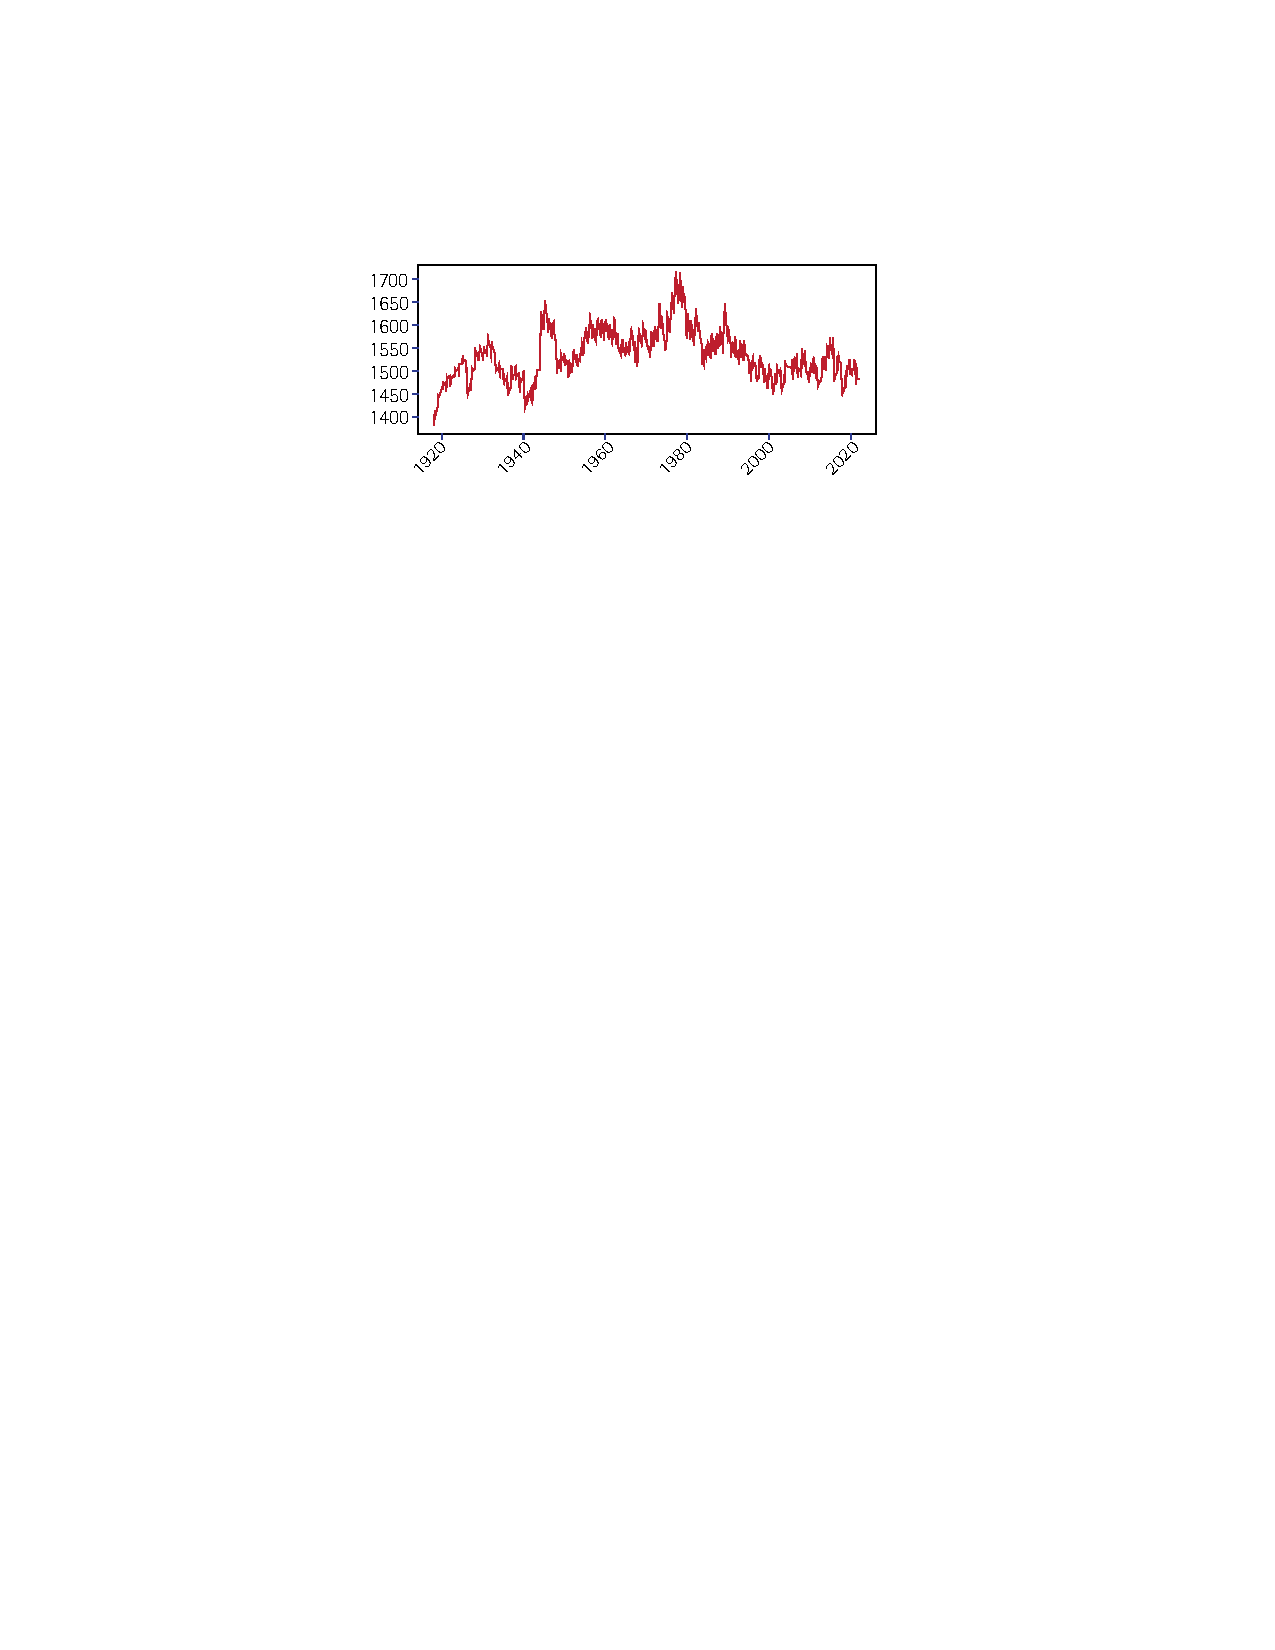
\includegraphics[width= 1\linewidth]{pic3}
		\caption{\small\textit{\color{toanhocdoisong}Hình $2$. Xếp hạng Elo của đội Montreal Canadiens từ năm $1917$ đến nay.}}
		\vspace*{-10pt}
	\end{figure}
	Ngoài ra, mô hình của Best và Paine tính đến cả hiệu số bàn thắng -- bàn thua của mỗi trận đấu và sự phụ thuộc lẫn nhau (hay tự tương quan) giữa các trận đấu liên tiếp.
	\vskip 0.05cm
	Hình $2$ cho thấy sự thay đổi của xếp hạng Elo của đội Montreal Canadiens theo mô hình của Best và Paine. Đỉnh cao nhất của đồ thị nằm ở nửa sau của thập niên $1970$, giai đoạn mà họ giành được bốn cúp Stanley\footnote[5]{\color{toanhocdoisong}Danh hiệu vô địch hàng năm của NHL -- Pi.}  liên tiếp.
	\vskip 0.05cm
	Ta cũng có thể thấy các đỉnh khác trong nửa sau thập niên $1940$ và giữa những năm $1990$, cũng như thời kỳ xuất sắc ổn định cuối những năm $1950$, khi họ vô địch năm lần liên tiếp (từ $1956$ đến $1960$). Trái lại, xếp hạng Elo của đội dao động quanh mức trung bình kể từ đầu những năm $2000$. Sự hiện diện của họ tại trận chung kết cúp Stanley năm $2021$, bởi vậy, có ít khả năng lặp lại trong tương lai gần.
	\vskip 0.05cm
	Vì xếp hạng Elo có tính tương đối, sẽ bổ ích hơn nếu ta so sánh sự thay đổi xếp hạng của các câu lạc bộ khác nhau. Hình $3$ so sánh các đội Montreal Canadiens (đường màu đỏ), Toronto Maple Leafs (xanh nước biển) và năm đội giành cúp Stanley từ $2008$ đến $2017$, gồm Boston Bruins (da cam), Detroit Red Wings (xanh lá cây), Chicago Blackhawks (đen), Los Angeles Kings (tím) và Pittsburgh Penguins (vàng).
	\begin{figure}[H]
		\vspace*{-10pt}
		\centering
		\captionsetup{labelformat= empty, justification=centering}
		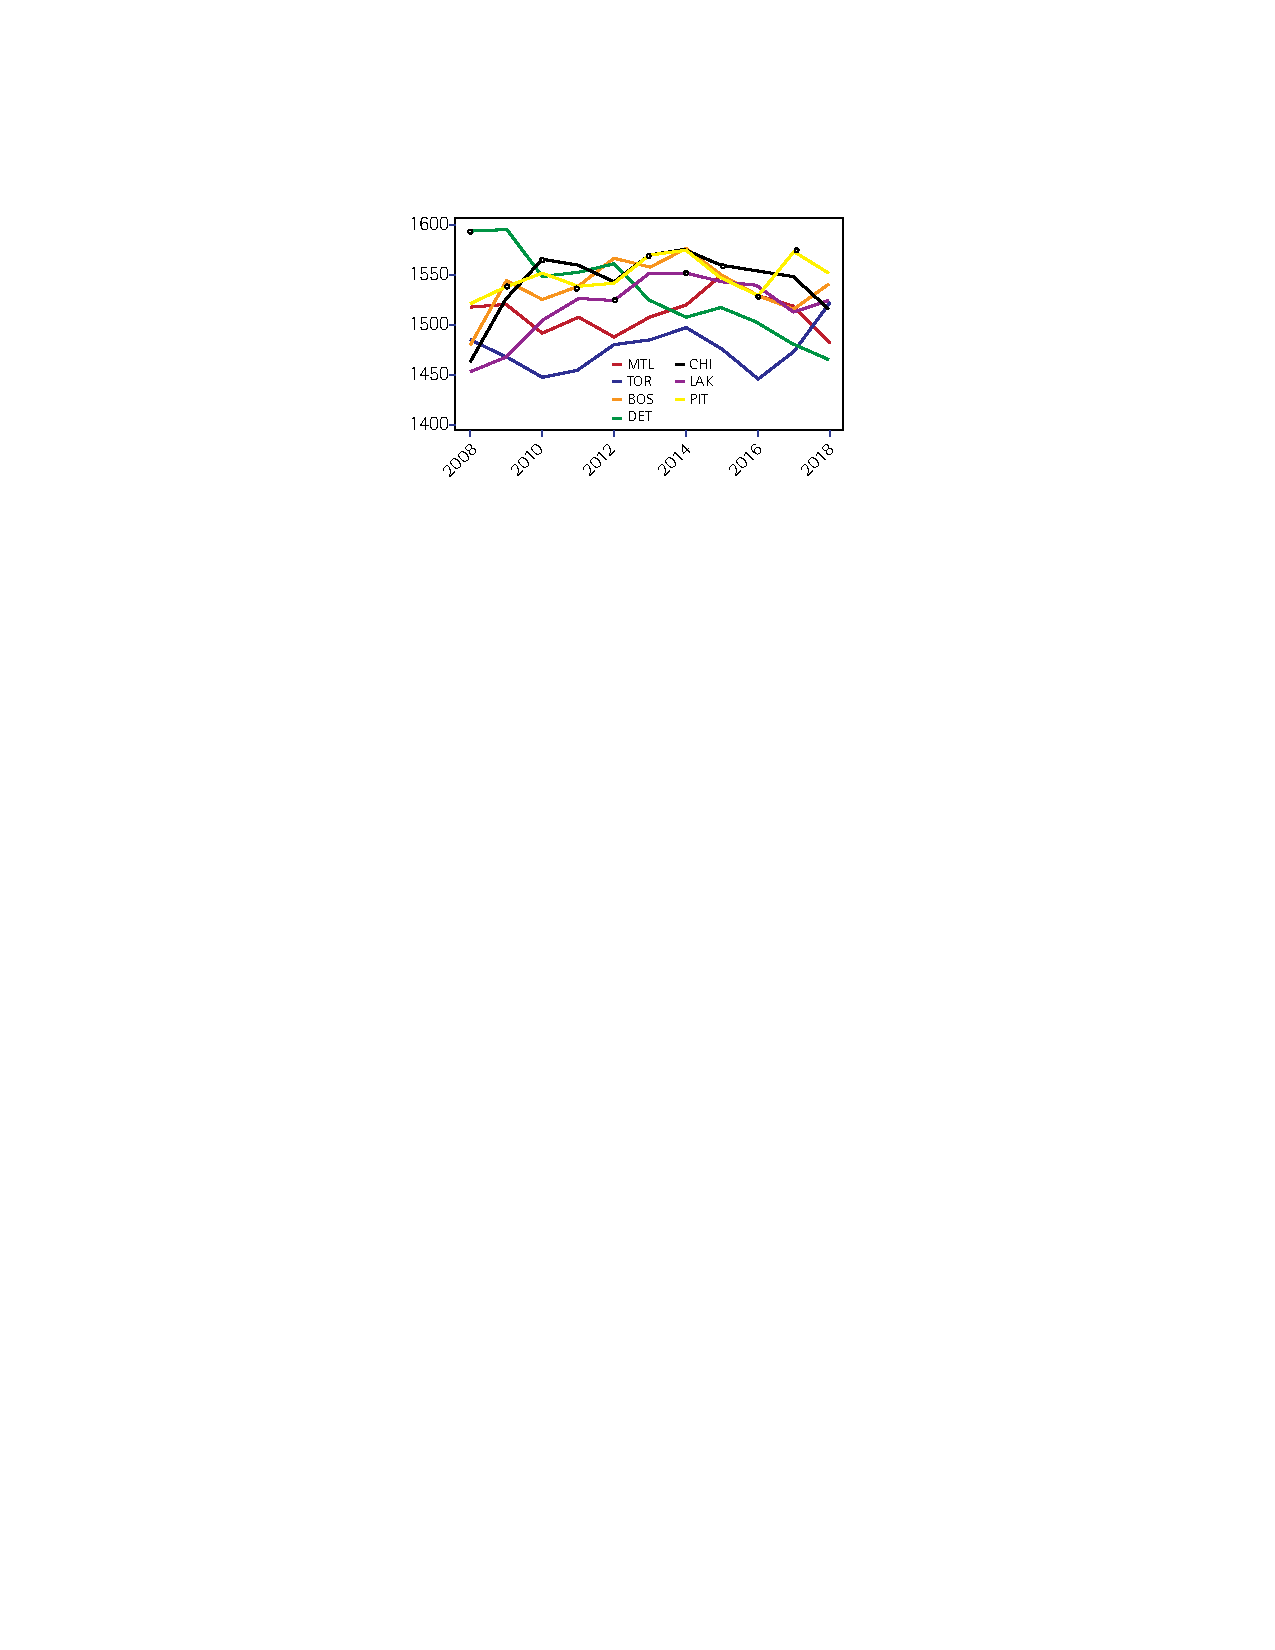
\includegraphics[width= 1\linewidth]{pic4}
		\caption{\small\textit{\color{toanhocdoisong}Hình $3$. Xếp hạng Elo của bảy đội NHL từ $2008$ đến $2018$; đội vô địch mỗi năm từ $2008$ đến $2017$ được đánh dấu bằng hình tròn.}}
		\vspace*{-10pt}
	\end{figure}
	Trong Hình $3$, các đội vô địch được đánh dấu bằng hình tròn. Đội vô địch năm $2018$, Washington Capitals, không được xét đến trong hình. Có thể thấy rõ là đội hay nhất không phải lúc nào cũng vô địch.
	\vskip 0.05cm
	\textbf{\color{toanhocdoisong}Kết luận}
	\vskip 0.05cm
	Là một yếu tố không thể thiếu trong thế giới cờ vua đồng thời có thể được áp dụng cho các trò chơi hai người có tổng bằng không nói chung, hệ thống tính điểm Elo cho phép đánh giá trình độ tương đối của các đấu thủ ngay cả khi họ chưa từng đối đầu nhau. Sự cập nhật liên tục dần dần qua từng trận đấu đem lại một cách đơn giản và hiệu quả để nắm bắt quá trình thay đổi của các đấu thủ hoặc của các đội, như được minh họa trong thí dụ về NHL.
	\vskip 0.05cm
	\PIbox{\textbf{\color{toanhocdoisong}Xếp hạng Elo của các kỳ thủ cờ vua}
		\vskip 0.05cm
		Ngày nay, một người mới chơi có điểm số Elo khoảng $1000$, còn một người chơi nghiệp dư giỏi có điểm số Elo khoảng $2000$. Các đại kiện tướng quốc tế cần đạt được điểm số Elo tối thiểu $2500$. Nhóm này gần như trùng với nhóm các kỳ thủ chuyên nghiệp, ngày nay có hơn $1000$ người trên toàn thế giới. Cho đến nay chỉ có khoảng mười lăm kỳ thủ từng đạt đến mức điểm Elo $2800$ trong sự nghiệp của mình.
		\vskip 0.05cm
		Các phần mềm cờ vua cũng có xếp hạng điểm Elo. Chương trình tốt nhất hiện nay, Stockfish, có điểm số Elo khoảng $3700$, cho thấy trong cờ vua máy tính đã vượt xa con người như thế nào: xác suất $p_{AB}$ giữa Stockfish ($A$) và Magnus Carlsen ($B$) là khoảng $0{,}992\ldots$ (tức là trung bình $992$ trận thắng và $8$ trận thua cho máy tính sau $1000$ trận đấu không có hòa). Đó cũng là khoảng cách giữa Carlsen và một kỳ thủ nghiệp dư giỏi có điểm số Elo $2000$, mức đạt được bởi khoảng $30000$ người.
		\vskip 0.05cm
		Ta cũng có thể đặt câu hỏi liệu xếp hạng Elo có thể g  iúp so sánh các kỳ thủ thuộc các thời đại khác nhau. Chẳng hạn, một kỳ thủ có điểm Elo $2700$ trong thập niên $1980$ liệu có trình độ tương đương với một kỳ thủ có điểm Elo $2700$ ngày nay? Đây là một câu hỏi phức tạp, nhất là khi bản thân môn cờ vua cũng đã thay đổi. Chẳng hạn, các kỳ thủ, từ những người chuyên nghiệp đến những người nghiệp dư hăng hái nhất, đều dùng phần mềm để luyện tập. Nhưng người ta cũng quan sát được hiện tượng ``lạm phát", được gây ra bởi chính cách tính điểm Elo. Từ đầu những năm $2000$, điểm Elo trung bình của $50$ kỳ thủ mạnh nhất đã tăng hàng chục điểm, do đó điểm Elo cỡ $2700$ ở năm $2010$ rất có thể kém giá trị hơn so với ở năm $2000$.}
\end{multicols}